\documentclass{article}
\usepackage{graphicx}
\graphicspath{ {images/} }
\title{Deep Q Learning for Rocket Landing}
\date{March 2018}
\author{Ibis Prevedello}

\begin{document}
\maketitle

\section{Introduction}
The goal of this project is to study and implement a Reinforcement Learning algorithm in order to solve several games from the Gym Toolkit \cite{gym}. The algorithm chosen is called Deep Q Learning, and uses a Deep Neural Network to learn the Q Function. Besides the implementation, also some improvements are tried with Double Deep Q Learning and Prioritized Experience Replay in order to improve performance.

\section{Description of the problem}
Besides the idea is to develop an algorithm that can be used for more than one game, this report will contain only the solution for the environment called 'Rocket Landing', which is inspired on SpaceX idea of reusable rockets.

\begin{figure}[h]
\centering
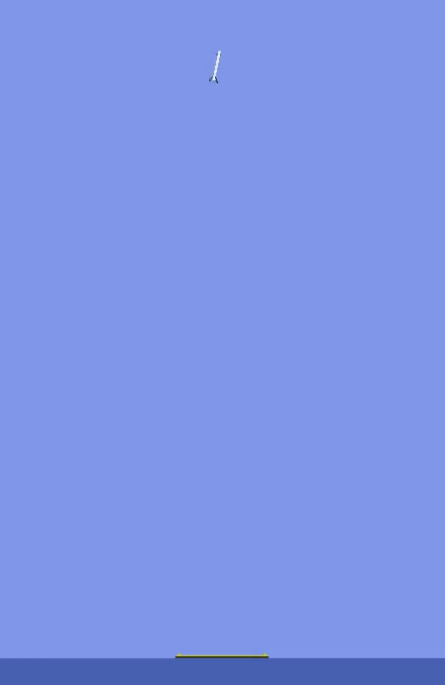
\includegraphics[scale=0.30]{environment}
\caption{Game screenshot}
\label{fig:fig1}
\end{figure}

The rocket starts from a high altitude, out of the screen, as shown in image \ref{fig:fig1}, and the goal is to control it using the trusters in order to land it on a drone on the sea. The landing also needs to occur smootly in order to avoid demaging the rocket legs.

\section{Formal model of the problem}
To control the rocket it is necessary to give to the learning algorithm the actual state of the problem, called state variables and take one of the actions from the control inputs.
After every iteration, which is a frame of the simulation, an action will be calculated and a result of that action will be returned to the algorithm as a reward and the result state.

\subsection{State variables}
For the state variables, it is possible to limit the number of variables used for the training, however it was decided to use all the data available in order to have a better control of the rocket.

\begin{itemize}
	\item x position
    \item y position
    \item angle
    \item first leg ground contact indicator
    \item second leg ground contact indicator
    \item throttle
    \item engine gimbal
	\item x velocity
    \item y velocity
    \item angular velocity
\end{itemize}

\subsection{Control inputs}
Using this simulator it is possible to chose one of the two types of controls, or discrete or continuous. It was decided to use discrete control because the same code could be used to a bigger variety of other simulators inside Gym.

\begin{itemize}
	\item gimbal left
    \item gimbal right
    \item throttle up
    \item throttle down
    \item use first control thruster
    \item use second control thruster
    \item no action
\end{itemize}

\subsection{Reward function}
The reward function for this environment envolves a series of variables, such as rocket's speed, distance to the goal, angle, angular velocity, fuel, ground contact and some other variables. It is only interesting to cite that the reward value improves as the rocket gets closer to the goal.

\section{Solution algorithm}
A algorithm well known is the Q Learning, which has the goal of finding a sequence of actions from some state that leads to a reward. Some actions may lead to a greater reward, others may achieve the goal faster.

The original Q Learning algorithm uses a table $Q(s,a)$, composed of rows of states and columns of actions. It uses the Bellman equation, which states that the expected long-term reward for a given action is equal to the immediate reward from the current action combined with the expected reward from the best future action taken at the following state.

\[Q(s,a)=r_0+\gamma(r_1+\gamma r_2+\gamma^2 r_3+...)=r_0+\gamma max_a Q(s',a)\]

In the case of this problem, because the states are constante, it is not possible to use a table, and it is substituted by a neural network. So the goal is to update the weights of the neural network, but it follows the same equation and the same process.

\subsection{Hyperparameters}
The hyperparameters used for this project are presented in the table below:

\begin{center}
\begin{tabular}{ |c|c| }
 \hline
 \textbf{Parameter} & \textbf{Value} \\ 
 \hline
 $\gamma$ (reward discount factor) & 0.99 \\ 
 learning rate & 0.00025 \\
 target update (episodes) & 1000 \\ 
 $\epsilon$ start & 1.0 \\ 
 $\epsilon$ end & 0.01 \\ 
 $\epsilon$ decay & 0.0001 \\ 
 batch size & 128 \\ 
 memory capacity & 200000 \\ 
 \hline
\end{tabular}
\end{center}

\subsection{Exploration and exploitation}
The way the algorithm chooses the action is called policy. A variable $\epsilon$ is used in order to help with this decision, at the beggining it is important to chose random actions in order to get a better felling about exactly what is the response of the system given an action, it is called exploration. As the iterations passes this $\epsilon$ decreases in order to fine tune the parameters, what is called exploitation.

\subsection{Experience replay}
It was achnowledged by the authors of the original paper that using only a neural network to represent the Q function make it unstable \cite{deepQLearning}.

When using online learning from each simulation step the problem is that the samples feed to the neural network are higly correlated, so the network will most likely overfit and fail to generalize properly.

The solution found is to store the last $n$ experiences in a memory and instead of training the network with only one sample use a random batch from this memory, as described in \cite{experienceReplay}.

\subsection{Double deep learning}

\subsection{Prioritize experience replay}

\section{Implementation}
The algorithm here described is divided in tree different parts, the memory, the brain and the agent. Each one has its own well defined role and it is important to keep the code separated and organized.

\subsection{Memory}
The memory is necessary to keep in memory a certain number of last actions executed by the agent. It is necessary to store the experience that will be used for Experience Replay.

The Experience Replay is a stratagy used to train the Neural Network not only based on the last experience, but on a batch with multiple experiences saved in the memory. For this part there are multiple ways to select this samples from the memory, random samples are one, and other more efficient algorithm is to determine an error for each sample and select those with a hier error.

Each experience saved to the memory have the following information:

\begin{itemize}
	\item current state
	\item action
	\item reward
	\item next state
\end{itemize}

\subsection{Brain}
The Brain class encapsulates the Neural Network. It was defined with 2 hidden layers with 256 neurons each and ReLU activation function. The input number of neurons is the number of states and the output number of neuros is the number of actions.

This network is trained in order to aproximate the Q function and the target model is a simple copy of the model, however it is updated sporadically, after 1000 steps.

For the loss it is using the Huber loss function, it is a loss function used in robust regression, that is less sensitive to outliers in data than the squared error loss.

\subsection{Agent}
The Agent class is a container that encapsulates all the methods for the algorithm to run, such as the act, observe, replay and epsilon decrement.

Also some more higher level tasks are also implemented like save and load model, which enables the script to stop training and continue it from where it stopped.

\section{Results}
The first data that is useful to analize is the evolution of rewards over the training. In image \ref{fig:fig2} is plotted this evolution and it is possible to see the the reward is improving over time, even though

\begin{figure}[h]
\centering
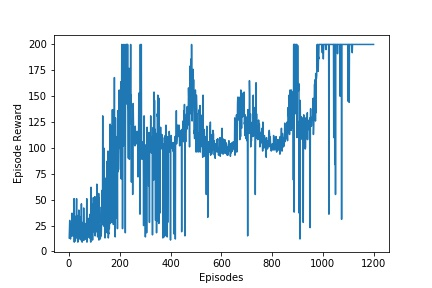
\includegraphics[scale=0.5]{rewardOverEpisodes}
\caption{Reward over episodes}
\label{fig:fig2}
\end{figure}

\section{Conclusions}
Another option 

\begin{thebibliography}{9}

\bibitem{deepQLearning} 
Mnih et al.
\textit{Human-level control through deep reinforcement learning}. 
Nature 518, 2015.

\bibitem{experienceReplay} 
Lin L.
\textit{Reinforcement Learning for Robots Using Neural Networks}. 
PhD. thesis, Carnegie Mellon University Pittsburgh, 1993.

\bibitem{gym} 
OpenAI Gym.
\\\texttt{https://github.com/openai/gym}

\end{thebibliography}

\end{document}